% Provides macros manipulating strings of tokens.
\RequirePackage{xstring}

% Store the jobname as a string with category 11 characters.
\edef\normaljobname{\expandafter\scantokens\expandafter{\jobname\noexpand}}
\StrBehind{\normaljobname}{exer-}[\exercisenumber]

\documentclass[
  coursecode={CMPE 251},
  assignmentname={Exercise \exercisenumber},
  studentnumber=20053722,
  name={Bryan Hoang},
  draft,
  % final,
]{
  ltxanswer%
}

\marksnotpoints{}

\usepackage{bch-style}

\begin{document}
  \begin{figure}
    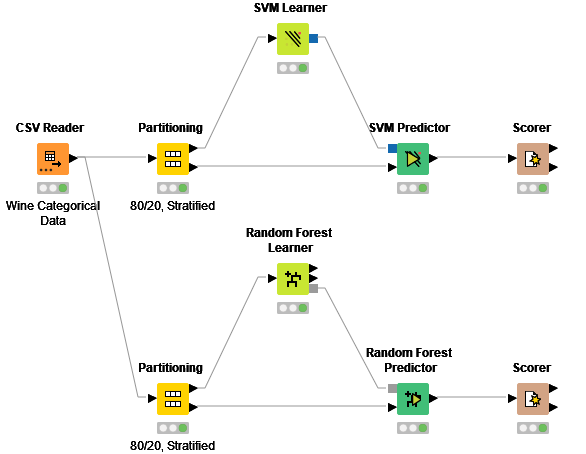
\includegraphics[width=\textwidth]{wine-workflow.png}
    \captionof{figure}{KNIME workflow used for SVM and RF analysis}\label{fig:wine-workflow-unnormalized}
  \end{figure}

  \begin{questions}
    \question[2]{}
    Try using a Support Vector Machine to predict the wine type. Experiment with both the C parameter (penalty for points inside the block) and the choice of kernel. Write a brief comment on which configuration performs best.
    \begin{solution}
      I tested all three kernel types, each with values of \(C\in\{0.1,1,10\}\).

      \section*{Kernel Type: Polynomial}
      I used degree 1 and degree 2 polynomial kernels, as seen in Figure~\ref{fig:wine-svm-p-1} and Figure~\ref{fig:wine-svm-p-2} respectively.

      \newpage

      \begin{answerfigure}
        \begin{subfigure}{0.49\textwidth}
          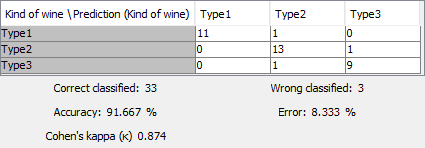
\includegraphics[width=\textwidth]{wine-svm-p-1-c-01.png}
          \caption{\(C=0.1\)}
        \end{subfigure}
        \begin{subfigure}{0.49\textwidth}
          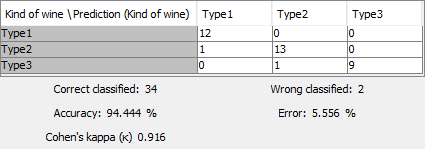
\includegraphics[width=\textwidth]{wine-svm-p-1-c-1.png}
          \caption{\(C=1\)}
        \end{subfigure}
        \par\bigskip
        \begin{subfigure}{0.49\textwidth}
          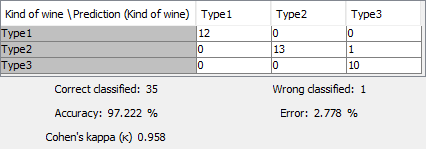
\includegraphics[width=\textwidth]{wine-svm-p-1-c-10.png}
          \caption{\(C=10\)}
        \end{subfigure}
        \caption{Confusion matrices of the SVM with degree 1 polynomial kernels}
        \label{fig:wine-svm-p-1}
      \end{answerfigure}
      \begin{answerfigure}
        \begin{subfigure}{0.49\textwidth}
          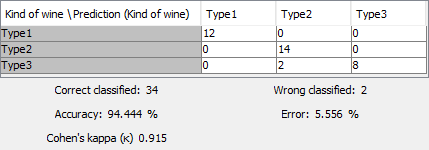
\includegraphics[width=\textwidth]{wine-svm-p-2-c-01.png}
          \caption{\(C=0.1\)}
        \end{subfigure}
        \begin{subfigure}{0.49\textwidth}
          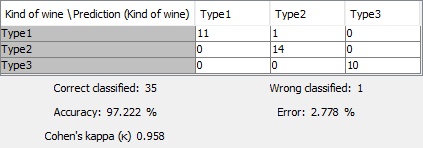
\includegraphics[width=\textwidth]{wine-svm-p-2-c-1.png}
          \caption{\(C=1\)}
        \end{subfigure}
        \par\bigskip
        \begin{subfigure}{0.49\textwidth}
          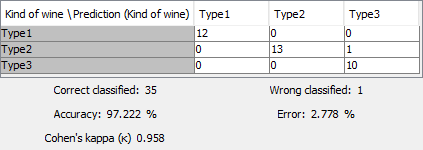
\includegraphics[width=\textwidth]{wine-svm-p-2-c-10.png}
          \caption{\(C=10\)}
        \end{subfigure}
        \caption{Confusion matrices of the SVM with degree 2 polynomial kernels}
        \label{fig:wine-svm-p-2}
      \end{answerfigure}
      Degree 3 and above polynomial kernels could not find support vectors.

      \section*{Kernel Type: Hyper Tangent}
      A Hyper Tangent kernel could not find support vectors.

      \section*{Kernel Type: Radial basis function (RBF)}
      For all values of \(C\in\{0.1,1,10\}\), the RBF kernel performed eactly the same, as seen in Figure~\ref{fig:wine-svm-rbf}.
      \begin{answerfigure}
        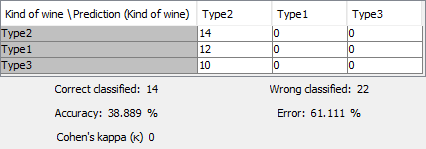
\includegraphics[width=0.5\textwidth]{wine-svm-rbf.png}
        \caption{Confusion matrix of the SVM with a RBF kernel}
        \label{fig:wine-svm-rbf}
      \end{answerfigure}

      \section*{Analysis}
      For the wine dataset, the SVM performed best with a polynomial kernel. From Figure~\ref{fig:wine-svm-p-1} and Figure~\ref{fig:wine-svm-p-2}, we can deduce that \textbf{an SVM with a degree 2 polynomial kernel and a \(C\) value of 10 performs the best among the tested configurations}.
    \end{solution}

    \newpage

    \question[2]{}
    Try the same prediction using a random forest. Don't be afraid to try a larger number of trees than the default.
    \begin{solution}
      I used a random forest (RF) with \(t\in\{50, 100, 150, 300, 500\}\) trees.
      \begin{answerfigure}
        \begin{subfigure}{0.49\textwidth}
          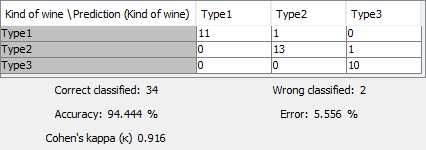
\includegraphics[width=\textwidth]{wine-svm-rf-50.png}
          \caption{\(t=50\)}
        \end{subfigure}
        \begin{subfigure}{0.49\textwidth}
          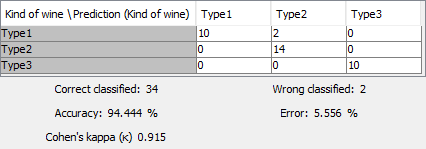
\includegraphics[width=\textwidth]{wine-svm-rf-100.png}
          \caption{\(t=100\)}
        \end{subfigure}
        \par\bigskip
        \begin{subfigure}{0.49\textwidth}
          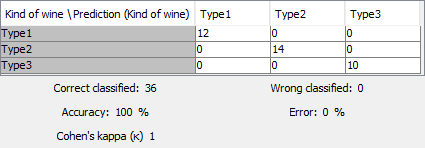
\includegraphics[width=\textwidth]{wine-svm-rf-150.png}
          \caption{\(t=150\)}
        \end{subfigure}
        \begin{subfigure}{0.49\textwidth}
          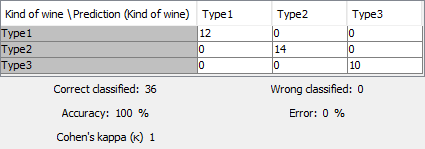
\includegraphics[width=\textwidth]{wine-svm-rf-300.png}
          \caption{\(t=300\)}
        \end{subfigure}
        \par\bigskip
        \begin{subfigure}{0.49\textwidth}
          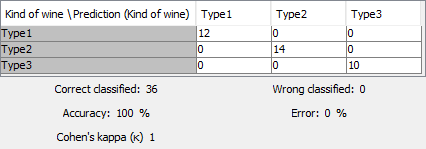
\includegraphics[width=\textwidth]{wine-svm-rf-500.png}
          \caption{\(t=500\)}
        \end{subfigure}
        \caption{Confusion matrices of the RF with varying number of trees}
        \label{fig:wine-svm-rf}
      \end{answerfigure}
      From Figure~\ref{fig:wine-svm-rf}, we can see that after hitting \(t=150\) trees, the RF performed perfectly on the dataset.
    \end{solution}
  \end{questions}
\end{document}
